\thispagestyle{empty}
\begin{center}
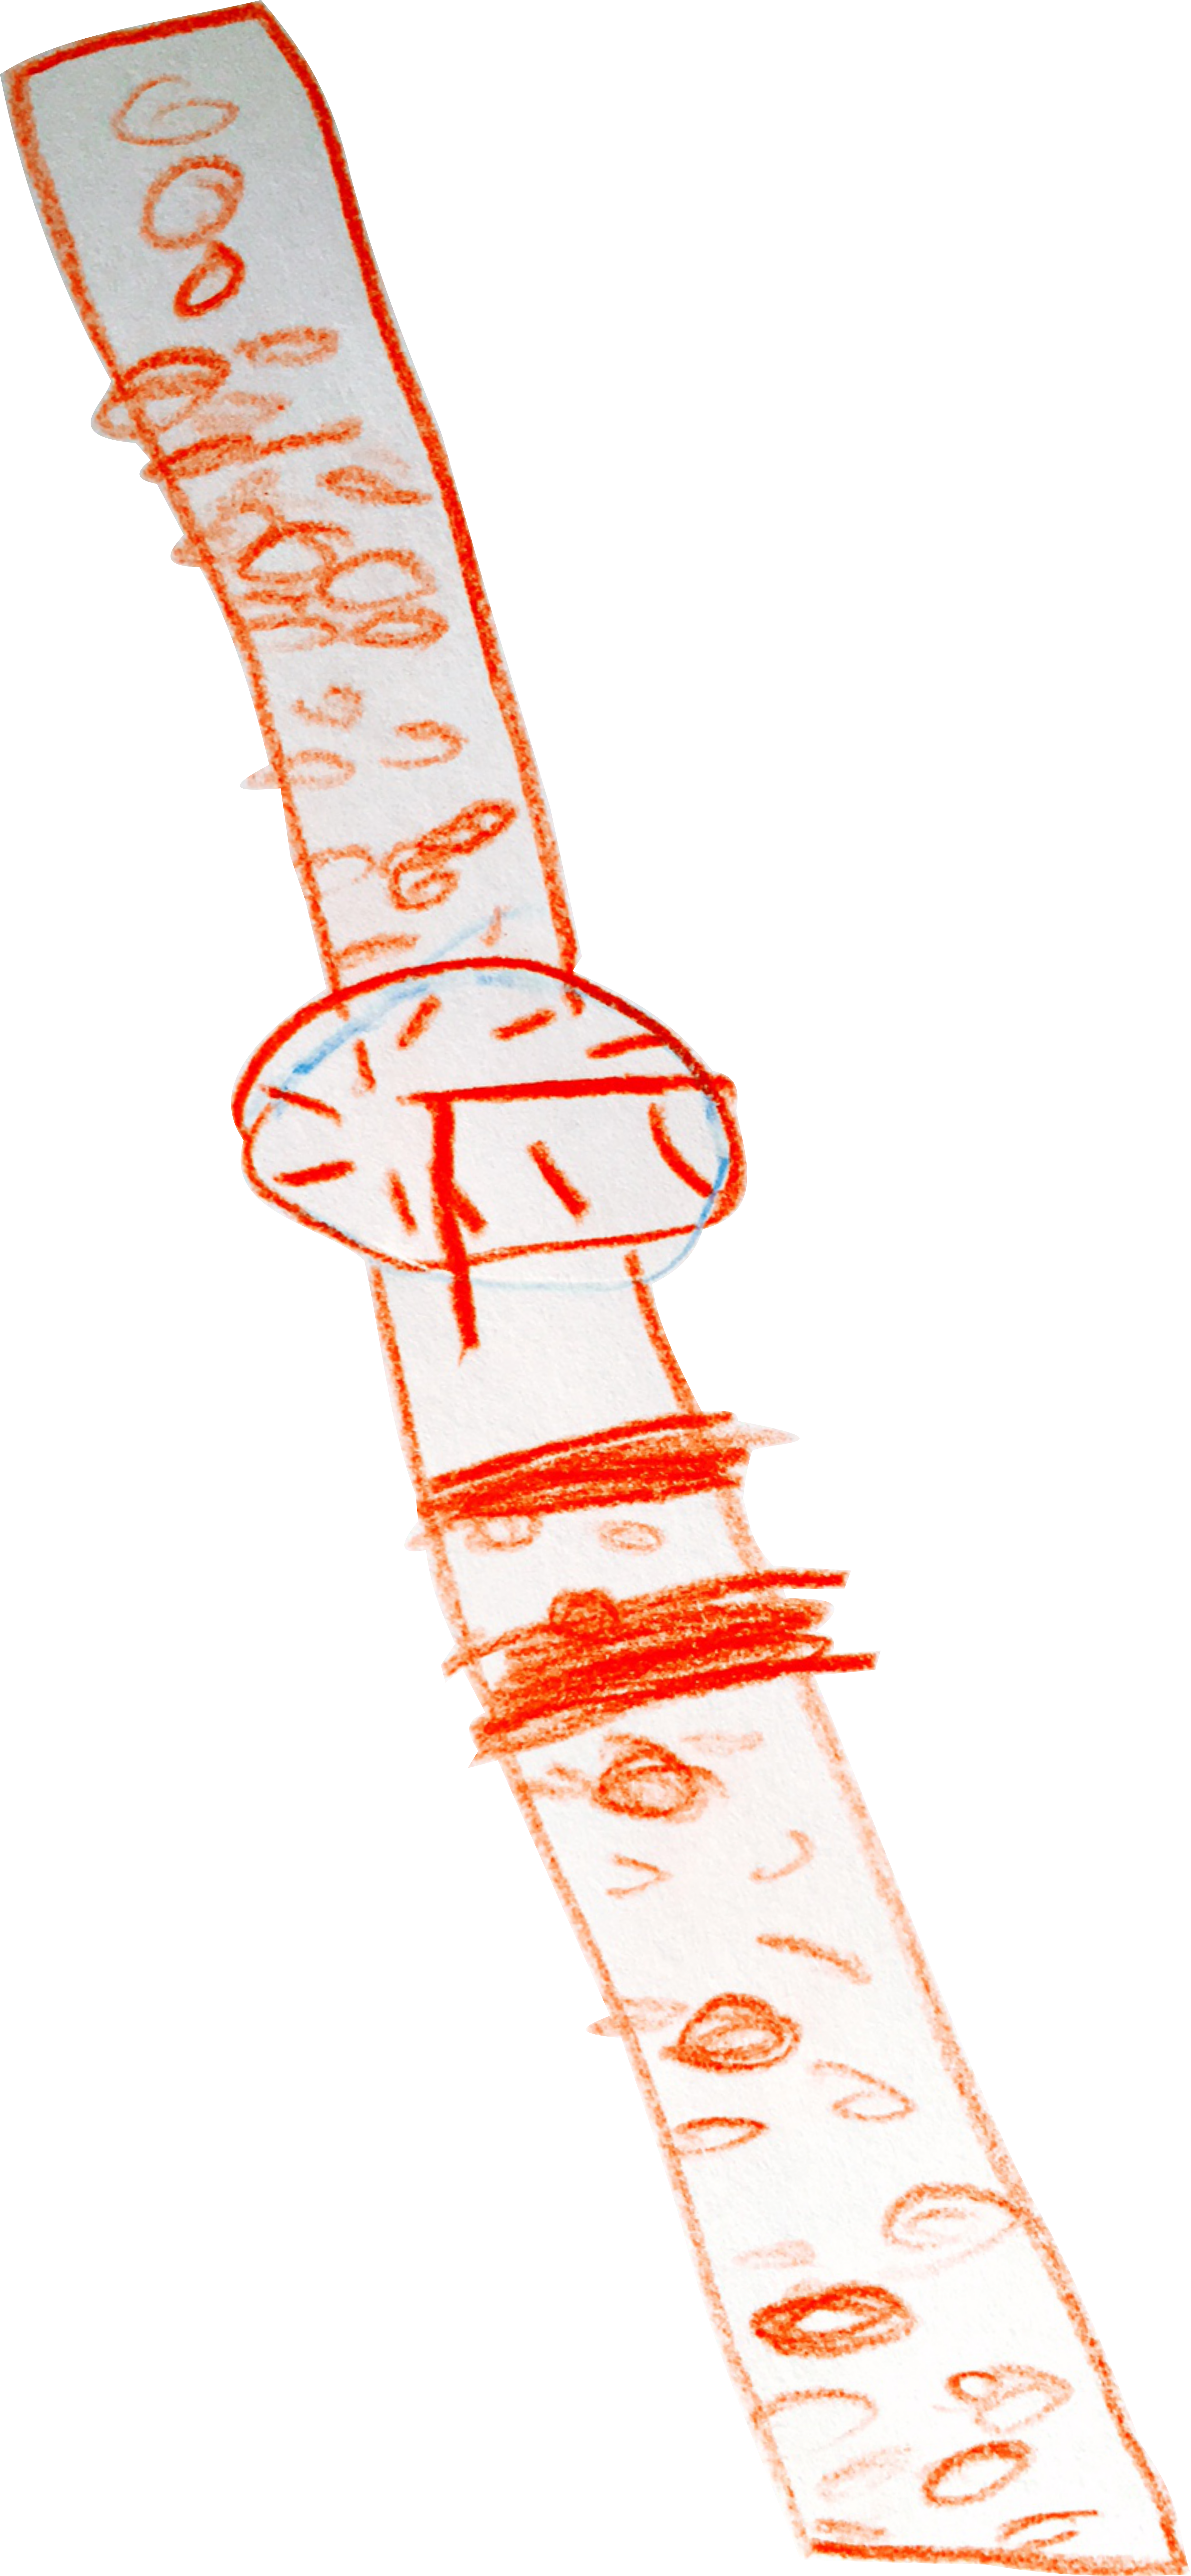
\includegraphics[height=.8\textheight]{./bilder/160120_uhr.png}
\end{center}
\vskip 2cm
{\Huge\color{farbe}\hfill{\ttfamily{Grüffelos Hunger}}}
\addcontentsline{toc}{chapter}{}
\newpage
%%%%%%%%%%%%%%%%%%%%%%%%%%%%%%%%%%%%%%%%%%%%%%%%%%%%%%%%%%%%%%%%%%%%%%%%%%%%%%%
\lettrine[lines=2, lhang=.2, loversize=.25, lraise=0.05, findent=0.1em,
nindent=0em]{A}{}
Der Grüffelo sitzt vor seiner Höhle. Sein Magen knurrt so laut, dass die Blätter in den Ästen wackeln. Und der Hunger ist nicht einmal das Schlimmst. Eine Maus hat ihn ausgetrickst. Ihn, den grossen und gefährlichen Grüffelo. Ihn, vor dem alle im Wald Angst haben. 

Na ja, vermutlichen Angst hatten. Nachdem die Maus ihm weiss gemacht hatte, dass sie so gefährlich und grauenhaft ist, dass sich sogar die Eule, die Schlange und der Fuchs vor ihr fürchten, hatte er schnell Reissaus genommen. Ein Reh hatte ihn auf seiner Flucht zu seiner Höhle gesehen. Und er, der mächtige Grüffelo hatte ihm im Vorbeirennen zugerufen, es solle sich in Acht nehmen, die Maus sei in diese Richtung unterwegs. 

Das Reh hatte sofort begriffen, was passiert war. Zum Haare ausraufen. Die Schadenfreude war natürlich riesig und noch schneller als er rennen konnte, hatte sich die Nachricht im ganzen Wald verbreitet. Und ein Grüffelo ist kein Grüffelo mehr, wenn ihn alle auslachen. Die gifitge Warze auf seiner Nase juckte gewaltig bei bei dem Gedanken. 

Drei Tage sitzt der Grüffelo jetzt schon in seiner Höhle und traut sich aus Scham nicht mehr heraus. Da ist es dunkel und kalt und niemand kann ihn sehen. So kann es nicht weiter gehen, denkt er sich. Wenigstens etwas essen muss ich. Immerhin ist er das gefährlichte Tier. Als er noch klein war, hatter er immer den Biber als Freund. Der war schlau, den könnte er jetzt fragen. Aber als ausgewachsener Grüffelo hat man keine Freunde. Alle fürchten einen.

Der Grüffelo kriecht aus seiner Höhle, putzt sich die Spinnweben ab und blinzelt in die Sonne. Die Augen sind so viel Licht gar nicht gewöhnt. Aber schon hört er ein Rascheln im Gebüsch. Das könnte ein Hase sein, leichte Beute also. Der grüffelo rennt mit einem lauten Schrei los und springt in die Richtung. Irgendetwas zieht aber plötzich seinen Kopf nach hinten und er landet krachend auf dem Boden. Er ist gegen einen Ast gelaufen, den er völlig übersehen hatte. Noch ganz durcheinander zieht er sich schnell in seine Höhle zurück, ganz nach hinten, bloss weit weg. Wenn das mal bloss niemand gesehen hat! Was wäre das für eine Schande.

\enquote{Grüffelo?}

Die Stimme kennt er. Das ist die Maus, die ihn so hereingelegt hat. Ausgerechnet.

\enquote{Alles in Ordnung bei Dir? Ich habe gesehen, wie du gegen den Baum gerannt bist.}

Zum ersten Mal seit vielen Jahren kullern dem Grüffelo dicke Tränen über die gefährlichen Hauer und die giftige Warze. 

\enquote{Nein, gar nichts ist in Ordnung. Alle lachen mich aus und Hunger habe ich auch.}

Der Grüffelo muss schluchzen.

\enquote{Na, na.}, sagt die kleine Maus.

\enquote{Das man auch einmal verliert, ist doch normal. Und gegen deinen Hunger weiss ich etwas. Probier doch mal einen von deinen Pilzen hier aus der Höhle.}



Dann eben so einen. Irgendetwas muss er jetzt essen. Aber wie gross ist seine Überraschung, dass der Pilz tatsächlich lecker ist! Er schmeckt ein wenig nach Erde, fast wie das Fleich eines Hirsches und gar nicht so grün und nach vielen Vitaminen wie die Pfalnzen und Beeren, die er so verachtet. Schmatzend isst er bis er so voll ist, dass er nur noch flach atmen kann.

Ab jetzt ist das Leben des Grüffelo ein anderes. Pilze wachsen in seiner Höhle mehr als genug. Er kann sie trocknen, kochen, braten, roh essen. Oder alles nacheinander. Und jeden Tag mühselig Tieren hinterher jagen muss er auch nicht mehr. Kein Fell mehr, das man erst abbekommen muss. 

Und noch etwas ist seitdem passiert. Die anderen Tiere des Waldes brauchten sich nicht mehr vor dem Grüffelo zu fürchten. Er konnte sich mit ihnen anfreunden. Besonders bei schlechtem Wetter oder im Winter war seine Höhle ein belibter Treffpunkt. 



\vfill



Der Grüffelo sitzt ganz allein
In seiner Höhle, Tag aus, Tag ein.
Die Sonne blinzelt von draussen herein,
aber Grüffelo will alleine sein.

Die Maus hat ihn herein gelegt,
Jetzt lacht der ganze Wald
Seitdem hat er sich nicht mehr bewegt
Verhungert hier sicher bald.

Der Magen knurrt das alles bebt
Aber sicher geht er nicht raus
er hat keine Freunde, wie er so lebt,
Nie besuch in seinem Haus

Ein Freund, der wäre jetzt wunderbar,
Eine Hilfe mit Rat und Tat

